\documentclass[conference,a4paper]{IEEEtran}

% ---------- Pacotes ----------------------------------------
\usepackage[T1]{fontenc}
\usepackage[utf8]{inputenc}
\usepackage{babel}
\babelprovide[import, main]{portuguese}
\usepackage{graphicx}
\usepackage{booktabs}
\usepackage{tabularx}
\usepackage{amsmath,amssymb}
\usepackage{enumitem}
\usepackage{microtype}
\usepackage[hidelinks]{hyperref}
\usepackage{cite}
\usepackage{stfloats}
\usepackage{float}

% Permite que floats de duas colunas ocupem até 90% do topo da página
\renewcommand{\dbltopfraction}{0.9}
\renewcommand{\dblfloatpagefraction}{0.9}

% ---------- Caminho das figuras ----------------------------
\graphicspath{{figures/}}

% ---------- Metadados --------------------------------------
\title{Sistema de Recuperação Rápida de Informações\\
       em Protocolos de Saúde do SUS\\
       {\large Relatório de Detalhamento}}

\author{
  \IEEEauthorblockN{Antônio Moreira Pinto, Celso Sacramento,
    João Pedro Porto Campos,\\Laura Gonzaga,
    Leonardo Sá Silveira Lima, Thiago Rocha}
  \IEEEauthorblockA{INF2921 / CIS2114 --- PUC-Rio\\
    Junho de 2026}
}

% ===========================================================
\begin{document}

\maketitle

\begin{abstract}
  Profissionais de saúde do SUS perdem tempo precioso buscando
  informações em protocolos clínicos distribuídos em PDFs
  fragmentados e sem indexação adequada. Este relatório detalha
  a proposta do Grupo~E: um assistente conversacional baseado em
  \textit{Retrieval-Augmented Generation} (RAG) que permite consultar
  protocolos em linguagem natural com respostas fundamentadas nas
  fontes oficiais. Neste relatório é detalhado o processo de concepção e construção inicial do sistema, assim como casos de uso e
  requisitos funcionais e não funcionais do sistema.
\end{abstract}

\IEEEpeerreviewmaketitle

% ---------- Seções -----------------------------------------

\section{Introdução}
\label{sec:intro}

O Sistema Único de Saúde (SUS) é operado por uma ampla rede de
profissionais que dependem de protocolos clínicos padronizados
para a tomada de decisão. Esses protocolos são distribuídos
majoritariamente em formato PDF, resultando em uma base documental
fragmentada e de difícil consulta durante o atendimento. A
dificuldade de acesso rápido a essas informações impacta diretamente
a qualidade e a velocidade do cuidado prestado ao paciente.

Este relatório apresenta o detalhamento inicial de um assistente
conversacional baseado em \textit{Retrieval-Augmented Generation}
(RAG) voltado a profissionais do SUS. As seções seguintes discutem
as soluções existentes (Seção~\ref{sec:related}), a arquitetura
proposta (Seção~\ref{sec:methods}), os requisitos iniciais
(Seção~\ref{sec:req}), os casos de uso ilustrativos
(Seção~\ref{sec:results}) e os resultados iniciais do protótipo
(Seção~\ref{sec:resultados}).

% ------------------------------------------------------------------

\section{Contexto e Soluções Existentes}
\label{sec:related}

Os Guias de Referência Rápida elaborados pelo Ministério da Saúde
e pelas Secretarias Municipais compilam critérios diagnósticos,
fluxos de atendimento e condutas terapêuticas~\cite{brasil2023protocolos}.
Entretanto, cada guia pode conter dezenas de páginas disponíveis
apenas em cópias físicas ou PDFs não indexados. Complementarmente,
o \textit{Data Zoom Saúde} disponibiliza microdados estruturados
do DATASUS que podem enriquecer respostas sobre indicadores e
disponibilidade de recursos~\cite{datazoom2024}.

As soluções existentes apresentam limitações relevantes. O
\textit{UpToDate} possui custo de licenciamento elevado e cobertura
limitada de protocolos do contexto brasileiro. O Telessaúde
não oferece interface conversacional e depende de consulta humana
assíncrona. Já os LLMs de uso geral não garantem
rastreabilidade até as fontes oficiais, gerando risco de respostas
desatualizadas ou incorretas~\cite{gao2023survey}.

A oportunidade identificada é combinar acesso conversacional com
fundamentação em documentos oficiais do SUS e integração com dados
estruturados, lacuna que o sistema proposto pretende preencher.

% ------------------------------------------------------------------

\section{Sistema Proposto}
\label{sec:methods}

\subsection{Visão Geral}

A solução é composta por três componentes integrados. O primeiro
realiza a extração e indexação dos Guias de Referência Rápida em
uma base vetorial, enriquecendo cada fragmento com metadados de
origem. O segundo conecta o sistema ao \textit{Data Zoom Saúde}
para recuperação de indicadores epidemiológicos estruturados. O
terceiro é a interface conversacional propriamente dita, que recebe
perguntas em linguagem natural, recupera os fragmentos mais
relevantes e gera respostas contextualizadas por meio de um LLM,
citando as fontes consultadas. A Figura~\ref{fig:mockup} ilustra
uma interação típica com o sistema na interface idealizada.

\begin{figure}[H]
  \centering
  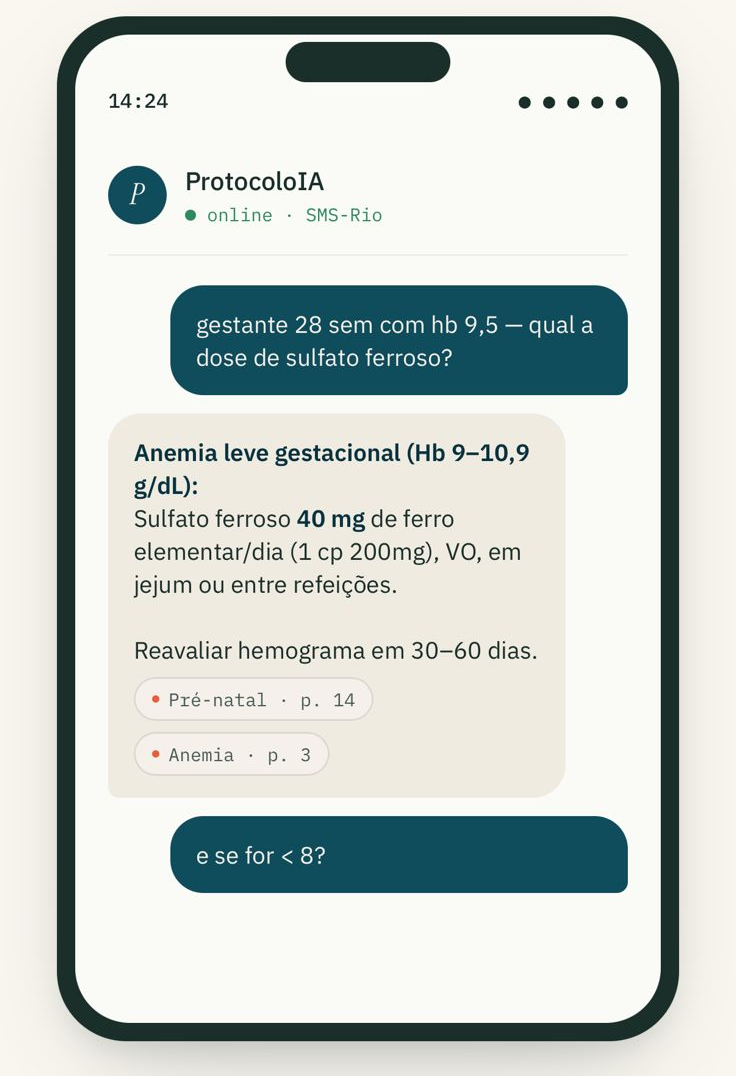
\includegraphics[width=0.6\columnwidth]{../figures/image.png}
  \caption{Mockup da interface conversacional do ProtocoloIA.}
  \label{fig:mockup}
\end{figure}

\subsection{Fontes de Dados}

O sistema opera sobre duas fontes complementares. Os Guias
de Referência Rápida (dado não estruturado) são documentos PDF
produzidos pelo Ministério da Saúde e Secretarias Municipais,
contendo fluxos clínicos e condutas terapêuticas. O \textit{Data
Zoom Saúde} (dado estruturado) oferece microdados do DATASUS
(SIH, SIA, SINAN) sobre produção ambulatorial, internações e
epidemiologia por município.

\subsection{Arquitetura de Recuperação}

O fluxo de consulta segue o padrão RAG~\cite{lewis2020rag}: a
pergunta do usuário é codificada em um vetor $\mathbf{q}$ e cada
fragmento indexado em um vetor $\mathbf{d}$, ambos produzidos por
um modelo de recuperação densa~\cite{karpukhin2020dpr}. Os $k$
fragmentos de maior similaridade do cosseno,

\begin{equation}
  \text{sim}(\mathbf{q}, \mathbf{d}) =
    \frac{\mathbf{q} \cdot \mathbf{d}}{\|\mathbf{q}\|\,\|\mathbf{d}\|},
  \label{eq:cosine}
\end{equation}

são concatenados ao prompt enviado ao LLM, que formula a resposta
final com referências explícitas às fontes consultadas.

O fluxo descrito foi implementado em um protótipo inicial, organizado em duas etapas: a ingestão, executada uma única vez por guia, e a geração, executada a cada pergunta do profissional.

Na etapa de ingestão, dois Guias de Referência Rápida foram utilizados como exemplo --- Diabetes Mellitus e Pré-Natal. Cada guia é dividido página a página, gerando em memória um PDF de página única para cada uma delas. Cada página é então vetorizada pelo modelo \texttt{gemini-embedding-2-preview}, escolhido por aceitar PDF como entrada e gerar o vetor a partir do texto, das tabelas, das imagens e do layout da página simultaneamente, dispensando a extração de texto como insumo direto para a vetorização, aspecto relevante para guias clínicos, ricos em fluxogramas e tabelas que um extrator de texto puro tende a perder. O texto da página também é extraído separadamente e mantido como reserva, mas não é o que alimenta o vetor. Os vetores resultantes são gravados em uma coleção persistente no \textit{Chroma}, acompanhados de metadados de origem (guia, caminho do arquivo e número da página), de modo que a etapa de ingestão, a mais onerosa, por exigir uma chamada de API por página, seja executada uma única vez por documento.

Na etapa de geração, a pergunta do profissional é codificada na mesma representação vetorial e utilizada para buscar, na coleção do Chroma, as $k$ páginas mais relevantes, com filtro opcional por guia. Os metadados das páginas recuperadas (arquivo e número da página) são então usados para localizar e recortar as páginas correspondentes no PDF original em disco; os bytes dessas páginas, em formato PDF, são enviados ao modelo multimodal \texttt{gemini-2.5-flash}, que lê a página diretamente e gera a resposta ao profissional. O conteúdo apresentado ao modelo é sempre relido do PDF original no momento da consulta já que o índice vetorial no Chroma serve apenas para localizar a página certa, não para fornecer o conteúdo da resposta. O \textit{prompt} instrui o modelo a citar explicitamente as páginas que fundamentam cada afirmação (no formato ``(pág.~N)'') e a indicar quando a resposta não está contida nas páginas fornecidas, evitando que o modelo complemente com conhecimento externo ao material recebido. O resultado é uma resposta acompanhada de referências que apontam para a página exata do guia correspondente, conforme ilustrado na Figura~\ref{fig:mockup}.

\begin{table*}[!t]
  \centering
  \caption{Requisitos funcionais do sistema.}
  \label{tab:req-func}
  \begin{tabularx}{\textwidth}{llX}
    \toprule
    \textbf{ID} & \textbf{Prior.} & \textbf{Descrição} \\
    \midrule
    RF01 & Alta  & Aceitar perguntas em português em linguagem natural, sem exigir conhecimento de sintaxe de busca. \\
    RF02 & Alta  & Recuperar trechos relevantes de PDFs indexados por meio de busca semântica baseada em similaridade vetorial. \\
    RF03 & Alta  & Gerar respostas fundamentadas nos documentos recuperados, citando o documento, seção e página de origem. \\
    RF04 & Alta  & Suportar múltiplos documentos PDF simultaneamente na base vetorial, com atualização incremental. \\
    RF05 & Alta  & Manter contexto de conversação em sessões curtas, permitindo perguntas de acompanhamento sem repetição. \\
    RF06 & Média & Integrar indicadores estruturados do \textit{Data Zoom Saúde} para enriquecer respostas com dados epidemiológicos. \\
    RF07 & Média & Exibir o trecho original do documento ao qual a resposta se refere, possibilitando verificação pela fonte. \\
    RF08 & Média & Indicar nível de confiabilidade da resposta com base na relevância dos fragmentos recuperados. \\
    RF09 & Baixa & Permitir filtragem de consultas por categoria de protocolo (ex.: imunização, saúde mental, hipertensão). \\
    RF10 & Baixa & Oferecer suporte a consultas por voz, convertendo fala em texto antes do processamento. \\
    \bottomrule
  \end{tabularx}
\end{table*}

\begin{table*}[!t]
  \centering
  \caption{Requisitos não funcionais do sistema.}
  \label{tab:req-nfunc}
  \begin{tabularx}{\textwidth}{llX}
    \toprule
    \textbf{ID} & \textbf{Categoria} & \textbf{Descrição} \\
    \midrule
    RNF01 & Usabilidade      & Interface acessível via browser sem instalação adicional, adequada a profissionais sem formação técnica. \\
    RNF02 & Rastreabilidade  & Toda resposta deve citar o documento fonte, seção e página, permitindo verificação e auditoria posterior. \\
    RNF03 & Segurança        & Dados clínicos identificáveis do paciente não devem ser incluídos nas consultas enviadas ao LLM nem nos logs. \\
    RNF04 & Confiabilidade   & O sistema deve indicar explicitamente quando não há informação suficiente nos documentos indexados. \\
    RNF05 & Escalabilidade   & A arquitetura deve suportar a inclusão de novos documentos sem reprocessamento total da base vetorial. \\
    RNF06 & Conformidade     & O sistema deve aderir à LGPD no tratamento de dados de acesso e de identificação de usuários. \\
    RNF07 & Manutenibilidade & Os documentos indexados devem poder ser atualizados independentemente, refletindo novas versões dos protocolos. \\
    \bottomrule
  \end{tabularx}
\end{table*}

% ------------------------------------------------------------------

\section{Requisitos do Sistema}
\label{sec:req}

A Tabela~\ref{tab:req-func} classifica os requisitos
funcionais por prioridade: alta prioridade compõe o núcleo do MVP a
ser validado na primeira iteração; média prioridade agrega valor sem
bloquear essa validação; baixa prioridade fica reservada para versões
subsequentes. A Tabela~\ref{tab:req-nfunc} organiza os requisitos não
funcionais por categoria de qualidade. Rastreabilidade e segurança
recebem atenção especial em razão das implicações clínicas do domínio
e da obrigação de conformidade com a LGPD.

% ------------------------------------------------------------------

\section{Casos de Uso}
\label{sec:results}

Foram elaborados 8 casos de uso da ferramenta, sendo os 3 primeiros elaborados pelo grupo e os outros 5 provenientes de entrevistas com 3 profissionais de saúde das áreas de Pediatria, Atendimento Intensivo e Clínica Geral:

\subsection{Caso de Uso 1: Consulta de Protocolo Clínico}

\begin{description}
  \item[Ator] Médico da Atenção Primária.
  \item[Objetivo] Confirmar a conduta terapêutica para hipertensão arterial sistêmica sem comorbidades durante o atendimento.
  \item[Pré-condição] Consulta médica em andamento; Guia de Referência Rápida da SMS indexado na base vetorial.
  \item[Cenário] Um médico da Atenção Primária, durante uma consulta, questiona o sistema sobre o protocolo de tratamento para hipertensão arterial sistêmica sem comorbidades. O assistente recupera os trechos pertinentes do Guia de Referência Rápida da SMS e apresenta a conduta recomendada com indicação da página e versão do documento, sem que o profissional precise interromper o atendimento para abrir o PDF manualmente.
  \item[Pós-condição] Conduta terapêutica obtida com página e versão do documento indicadas, sem interrupção do atendimento.
  \item[Requisitos relacionados] RF01, RF02, RF03, RF07, RNF01, RNF02.
\end{description}

\subsection{Caso de Uso 2: Consulta do Calendário de Vacinação}

\begin{description}
  \item[Ator] Enfermeira de UBS.
  \item[Objetivo] Confirmar o esquema vacinal de uma criança sem cartão de vacinação.
  \item[Pré-condição] Criança de 15 meses presente na unidade, sem cartão de vacinação; calendário vigente do PNI indexado.
  \item[Cenário] Uma enfermeira de UBS precisa confirmar o esquema vacinal para uma criança de 15 meses que chegou sem cartão de vacinação. Ao descrever a situação ao assistente, recebe uma lista estruturada das vacinas indicadas pelo Programa Nacional de Imunizações (PNI), com doses, vias de administração e intervalos mínimos, referenciada à versão vigente do calendário oficial.
  \item[Pós-condição] Lista estruturada de vacinas indicadas, com doses, vias e intervalos, obtida e referenciada à versão vigente.
  \item[Requisitos relacionados] RF01, RF02, RF03, RF07.
\end{description}

\subsection{Caso de Uso 3: Apoio à Decisão sobre Manual Clínico de Pré-Natal}

\begin{description}
  \item[Ator] Gestor municipal de saúde.
  \item[Objetivo] Definir, entre manuais clínicos de municípios distintos, qual adotar, usando a taxa de mortalidade materna como critério de comparação.
  \item[Pré-condição] Integração do sistema com o Data Zoom Saúde disponível; dados de nascidos vivos e óbitos maternos disponíveis para os municípios consultados.
  \item[Cenário] Um gestor municipal de saúde deseja decidir qual Manual Clínico de Pré-Natal adotar e pergunta ao sistema: ``Entre os municípios do Rio de Janeiro, São Paulo e Belo Horizonte, qual possui menor taxa de mortalidade materna?''. O sistema consulta os dados do Data Zoom Saúde via MCP, identifica a quantidade de nascidos vivos e de óbitos maternos nos municípios indicados e retorna a taxa de mortalidade materna calculada para cada um. O gestor utiliza essa taxa como um dos critérios para escolher o manual clínico do município com melhor indicador.
  \item[Pós-condição] Taxas de mortalidade materna por município retornadas; gestor utiliza o indicador como critério de decisão sobre o manual a adotar.
  \item[Requisitos relacionados] RF06.
\end{description}

\subsection{Caso de Uso 4: Estado Hiperosmolar Hiperglicêmico}

\begin{description}
  \item[Ator] Médico.
  \item[Objetivo] Confirmar a conduta para paciente com estado hiperosmolar hiperglicêmico.
  \item[Pré-condição] Atendimento em curso; Guia de Referência Rápida de Diabetes Mellitus indexado.
  \item[Cenário] Um médico relata o caso de um paciente de 47 anos com estado hiperosmolar hiperglicêmico e consulta o sistema durante o atendimento para confirmar a conduta indicada. O assistente recupera as páginas do Guia de Referência Rápida de Diabetes Mellitus que tratam da condição e apresenta a conduta recomendada, indicando a página de origem para verificação.
  \item[Pós-condição] Conduta recomendada obtida, com página de origem indicada.
  \item[Requisitos relacionados] RF01, RF02, RF03, RF07.
\end{description}

\subsection{Caso de Uso 5: Cetoacidose Diabética Sintomática}

\begin{description}
  \item[Ator] Médico.
  \item[Objetivo] Confirmar a conduta para cetoacidose diabética sintomática com dor abdominal e periférica.
  \item[Pré-condição] Atendimento em curso; Guia de Referência Rápida de Diabetes Mellitus indexado.
  \item[Cenário] Um médico questiona o sistema sobre o manejo de um quadro de cetoacidose diabética sintomática, com dor abdominal e dor periférica. O assistente recupera as páginas pertinentes do Guia de Referência Rápida de Diabetes Mellitus e apresenta a conduta recomendada, indicando a página de origem para verificação.
  \item[Pós-condição] Conduta recomendada obtida, com página de origem indicada.
  \item[Requisitos relacionados] RF01, RF02, RF03, RF07, RNF04.
\end{description}

\subsection{Caso de Uso 6: Poliúria em Paciente com Diabetes Tipo 2}

\begin{description}
  \item[Ator] Médico.
  \item[Objetivo] Investigar conduta para poliúria em paciente com diabetes tipo 2.
  \item[Pré-condição] Atendimento em curso; Guia de Referência Rápida de Diabetes Mellitus indexado.
  \item[Cenário] Um médico consulta o sistema sobre a investigação de poliúria em uma paciente de 63 anos com diabetes tipo 2. O assistente recupera as páginas pertinentes do Guia de Referência Rápida de Diabetes Mellitus e apresenta a conduta recomendada, indicando a página de origem para verificação.
  \item[Pós-condição] Conduta recomendada obtida, com página de origem indicada.
  \item[Requisitos relacionados] RF01, RF02, RF03, RF07.
\end{description}

\subsection{Caso de Uso 7: Abortamento com Sangramento}

\begin{description}
  \item[Ator] Profissional de saúde.
  \item[Objetivo] Confirmar a conduta diante de abortamento com sangramento em gestante.
  \item[Pré-condição] Atendimento em curso; Guia de Referência Rápida de Pré-Natal indexado.
  \item[Cenário] Um profissional consulta o sistema sobre o manejo de um processo de abortamento com sangramento em uma gestante de 24 anos. O assistente recupera os trechos pertinentes do Guia de Referência Rápida de Pré-Natal, apresenta a conduta indicada e a página correspondente, apoiando a decisão clínica sem que o profissional precise localizar manualmente a seção do guia.
  \item[Pós-condição] Conduta indicada obtida, com página correspondente, sem busca manual no guia.
  \item[Requisitos relacionados] RF01, RF02, RF03, RF07.
\end{description}

\subsection{Caso de Uso 8: Infecção Urinária em Gestante}

\begin{description}
  \item[Ator] Profissional de saúde.
  \item[Objetivo] Confirmar a conduta diante de infecção urinária em gestante.
  \item[Pré-condição] Atendimento em curso; Guia de Referência Rápida de Pré-Natal indexado.
  \item[Cenário] Um profissional consulta o sistema sobre a conduta diante de uma infecção urinária em uma gestante de 31 anos. O assistente recupera os trechos pertinentes do Guia de Referência Rápida de Pré-Natal, apresenta a conduta indicada e a página correspondente, apoiando a decisão clínica sem que o profissional precise localizar manualmente a seção do guia.
  \item[Pós-condição] Conduta indicada obtida, com página correspondente, sem busca manual no guia.
  \item[Requisitos relacionados] RF01, RF02, RF03, RF07.
\end{description}

% ------------------------------------------------------------------

\section{Resultados Iniciais}
\label{sec:resultados}

A partir das entrevistas realizadas com os profissionais de
saúde, além de elaborar os casos de uso apresentados
anteriormente, utilizamos as perguntas sugeridas pelos médicos
como teste do sistema. A seguir são apresentadas as respostas
dadas.

\subsection{Resultado 1: Estado Hiperosmolar Hiperglicêmico}

\noindent\textit{Pergunta:} ``Estou com um paciente homem de 47
anos com estado hiperosmolar hiperglicêmico, como posso
proceder?''

\medskip
\noindent\textit{Resposta do sistema:}

Para um paciente homem de 47 anos com estado hiperosmolar
hiperglicêmico (Síndrome Hiperglicêmica Hiperosmolar Não
Cetótica - SHH), deve-se proceder da seguinte forma:

\begin{enumerate}
  \item \textbf{Tratamento imediato:}
  \begin{itemize}
    \item Correção da desidratação, dos distúrbios eletrolíticos
          e da hiperosmolaridade sérica (pág. 101).
    \item Correção da hiperglicemia (pág. 101).
    \item Identificação e tratamento dos fatores precipitantes
          (pág. 101).
  \end{itemize}
  \item \textbf{Encaminhamento:}
  \begin{itemize}
    \item Em caso de suspeita de SHH, solicitar Vaga Zero para
          confirmação do diagnóstico e internação (pág. 101).
  \end{itemize}
\end{enumerate}

A SHH é uma complicação grave do diabetes mellitus, caracterizada
por hiperglicemia severa (glicemia superior a 600mg/dL),
hiperosmolaridade (osmolaridade sérica efetiva superior a
320mOsm/L) e desidratação, na ausência de cetoacidose (pH > 7,3
e bicarbonato > 18mEq/L) (pág. 99, 100). Hipercalemia também é
frequente (pág. 100). Tipicamente ocorre em adultos e idosos com
DM tipo 2 (pág. 100).

Os sinais e sintomas relacionados à hiperglicemia e ao aumento da
osmolaridade sérica incluem poliúria, polidipsia, fraqueza,
turvação visual e declínio progressivo do nível de consciência.
Em quadros mais graves, podem ocorrer sintomas neurológicos
focais, convulsões, hipotensão, choque e/ou insuficiência renal
aguda (pág. 100). Fatores precipitantes comuns são quadros
infecciosos, eventos cardiovasculares, patologias agudas clínicas
ou cirúrgicas e uso de certos medicamentos (pág. 100).

\textit{Fontes:}
\begin{itemize}
  \item {Guia Rápido Diabetes} --- pág. 49 (score=0.5241)
  \item {Guia Rápido Diabetes} --- pág. 100 (score=0.5360)
  \item {Guia Rápido Diabetes} --- pág. 101 (score=0.5424)
  \item {Guia Rápido Diabetes} --- pág. 8 (score=0.5506)
  \item {Guia Rápido Diabetes} --- pág. 98 (score=0.5508)
  \item {Guia Rápido Diabetes} --- pág. 102 (score=0.5548)
  \item {Guia Rápido Diabetes} --- pág. 62 (score=0.5576)
  \item {Guia Rápido Diabetes} --- pág. 47 (score=0.5626)
  \item {Guia Rápido Pré Natal} --- pág. 78 (score=0.5629)
  \item {Guia Rápido Diabetes} --- pág. 64 (score=0.5680)
\end{itemize}

\medskip
\noindent\textit{Observações:} esta foi a única das cinco
consultas em que o número de páginas recuperadas precisou ser
ampliado (de $k=5$ para $k=10$) para que a resposta cobrisse
adequadamente o quadro clínico; nota-se também a recuperação de
uma página do Guia de Pré-Natal (pág. 78) sem relação direta com
a pergunta, não utilizada na resposta final.

\subsection{Resultado 2: Cetoacidose Diabética Sintomática}

\noindent\textit{Pergunta:} ``Como proceder com um paciente com
cetoacidose sintomática com fortes dores abdominais e na região
periférica?''

\medskip
\noindent\textit{Resposta do sistema:}

Um paciente com cetoacidose sintomática e fortes dores abdominais
apresenta sinais que indicam a possibilidade de Cetoacidose
Diabética (CAD), uma complicação grave que exige remoção imediata
para unidades de emergência (pág. 97).

Deve-se proceder com:
\begin{itemize}
  \item \textbf{Encaminhamento imediato:} A dor abdominal é um
        dos sintomas que indicam a possibilidade de CAD, exigindo
        encaminhamento imediato ao serviço de emergência. Em caso
        de suspeita de CAD, deve-se solicitar Vaga Zero para
        confirmação do diagnóstico e internação (pág. 99). Se a
        glicemia capilar for maior ou igual a 300mg/dL, deve-se
        considerar Vaga Zero (pág. 111).
  \item \textbf{Tratamento:} As diretrizes de tratamento para CAD
        incluem (pág. 99):
  \begin{itemize}
    \item Manutenção das vias aéreas pérvias;
    \item Correção da desidratação;
    \item Correção dos distúrbios eletrolíticos e acidobásicos;
    \item Redução da hiperglicemia e da osmolalidade;
    \item Identificação e tratamento do fator precipitante.
  \end{itemize}
\end{itemize}

As páginas fornecidas não contêm informações específicas sobre
como proceder com dor na região periférica em casos de
cetoacidose sintomática.

\textit{Fontes:}
\begin{itemize}
  \item {Guia Rápido Diabetes} --- pág. 100 (score=0.5029)
  \item {Guia Rápido Diabetes} --- pág. 112 (score=0.5383)
  \item {Guia Rápido Diabetes} --- pág. 98 (score=0.5395)
  \item {Guia Rápido Diabetes} --- pág. 8 (score=0.5423)
  \item {Guia Rápido Diabetes} --- pág. 49 (score=0.5497)
\end{itemize}

\medskip
\noindent\textit{Observações:} o sistema sinaliza explicitamente
a ausência de informação sobre a dor periférica relatada na
pergunta, em vez de extrapolar além do material indexado,
ilustrando o comportamento esperado pelo requisito RNF04.

\subsection{Resultado 3: Poliúria em Paciente com Diabetes Tipo 2}

\noindent\textit{Pergunta:} ``Como proceder com uma paciente
mulher, 63 anos, diabética tipo 2, que está com quadro de
poliúria?''

\medskip
\noindent\textit{Resposta do sistema:}

Com base nas páginas anexadas, a poliúria é um sintoma típico de
DM2 e um sintoma de hiperglicemia aguda/insulinopenia (pág. 48,
pág. 62).

Nesse caso, a conduta deve ser:
\begin{enumerate}
  \item \textbf{Avaliar o início de insulina e individualizar o
        plano de cuidado} (pág. 48).
  \item \textbf{Iniciar insulina NPH} na dose de 10UI (0,2UI/kg)
        antes de deitar. Deve-se \textbf{manter a sulfonilureia e
        a metformina}, se o paciente já estiver em uso e não
        houver contraindicação (pág. 62).
  \item \textbf{Aferir a glicemia capilar em jejum para ajuste},
        realizando ajustes a cada 3 dias até alcançar a meta
        (pág. 62). Se a dose noturna for maior que 30UI,
        fracionar (metade antes do café e metade antes de
        deitar), suspender a sulfonilureia e manter a metformina
        (pág. 62).
\end{enumerate}

É importante notar que a poliúria também é mencionada como um
sintoma de descompensação do diabetes (pág. 22). Embora as
páginas mencionem a poliúria em contextos de emergência como CAD
(Cetoacidose Diabética) em pacientes com glicemias >200mg/dL
(pág. 99), a pergunta foca na poliúria como sintoma em uma
paciente já diagnosticada com DM2, o que, conforme as figuras,
leva à avaliação e início de insulina.

\textit{Fontes:}
\begin{itemize}
  \item {Guia Rápido Diabetes} --- pág. 49 (score=0.5096)
  \item {Guia Rápido Diabetes} --- pág. 63 (score=0.5123)
  \item {Guia Rápido Diabetes} --- pág. 23 (score=0.5271)
  \item {Guia Rápido Diabetes} --- pág. 100 (score=0.5314)
  \item {Guia Rápido Diabetes} --- pág. 22 (score=0.5320)
\end{itemize}

\medskip
\noindent\textit{Observações:} o sistema diferenciou
corretamente o quadro de poliúria como sintoma de descompensação
crônica do quadro de poliúria em contexto de emergência (CAD),
justificando explicitamente a interpretação escolhida com base na
ausência de outros sinais de emergência na pergunta.

\subsection{Resultado 4: Abortamento com Sangramento}

\noindent\textit{Pergunta:} ``Como proceder com uma paciente
mulher de 24 anos, gestante, que está passando por um processo de
abortamento com extravasamento sanguíneo?''

\medskip
\noindent\textit{Resposta do sistema:}

Para uma paciente gestante de 24 anos que está passando por um
processo de abortamento com extravasamento sanguíneo, a conduta
é:
\begin{enumerate}
  \item \textbf{Em caso de ``Trabalho de abortamento''}
        (caracterizado por sangramento vaginal ativo, colo
        entreaberto ou dilatado, com ou sem dor), a gestante deve
        ser encaminhada via Vaga Zero para a emergência
        obstétrica. Se a gestação for até 12 semanas, o
        encaminhamento é via SISREG (pág. 24).
  \item \textbf{Se for um ``Abortamento incompleto''} (com
        sangramento mais volumoso que na ameaça de abortamento,
        dores intensas e orifício do colo uterino aberto), a
        conduta é encaminhar para avaliação via Vaga Zero
        (pág. 134).
  \item \textbf{Se for uma ``Ameaça de abortamento''} (com
        sangramento genital de intensidade pequena a moderada,
        volume uterino compatível com a idade gestacional e
        orifício do colo uterino fechado), deve-se considerar a
        necessidade de encaminhar para avaliação em maternidade
        via Vaga Zero, solicitar USG, manter a gestante em
        repouso, evitar relações sexuais e avaliar a necessidade
        de analgésicos em caso de dor significativa (pág. 133).
  \item \textbf{Em caso de ``Abortamento retido''} ou
        \textbf{``Abortamento infectado''}, também se deve
        encaminhar para avaliação via Vaga Zero (pág. 134).
\end{enumerate}

Dado que a paciente está ``passando por um processo de
abortamento com extravasamento sanguíneo'', a conduta mais
provável e urgente, de acordo com as páginas fornecidas, é o
\textbf{encaminhamento para avaliação via Vaga Zero para a
emergência obstétrica} (pág. 24, 134), a menos que se confirme
ser um abortamento completo e não haja sinais de complicação.

\textit{Fontes:}
\begin{itemize}
  \item {Guia Rápido Pré Natal} --- pág. 134 (score=0.4963)
  \item {Guia Rápido Pré Natal} --- pág. 135 (score=0.5189)
  \item {Guia Rápido Pré Natal} --- pág. 25 (score=0.5195)
  \item {Guia Rápido Pré Natal} --- pág. 136 (score=0.5424)
  \item {Guia Rápido Pré Natal} --- pág. 19 (score=0.5577)
\end{itemize}

\medskip
\noindent\textit{Observações:} o sistema cobriu as quatro
classificações de abortamento previstas no guia antes de
concluir pela conduta mais provável dado o quadro descrito,
explicitando a ressalva de que a confirmação do tipo exato de
abortamento poderia alterar o encaminhamento.

\subsection{Resultado 5: Infecção Urinária em Gestante}

\noindent\textit{Pergunta:} ``Como proceder com uma paciente
mulher de 31 anos, gestante, que está com infecção urinária?''

\medskip
\noindent\textit{Resposta do sistema:}

Para proceder com uma paciente mulher de 31 anos, gestante, com
infecção urinária (cistite aguda), deve-se considerar o seguinte,
com base nas páginas fornecidas:

\begin{enumerate}
  \item \textbf{Diagnóstico e Início do Tratamento:}
  \begin{itemize}
    \item A cistite aguda é caracterizada por sintomas como
          disúria, polaciúria, incontinência urinária, dor
          suprapúbica e hematúria. Não deve haver febre,
          taquicardia, dor abdominal intensa, dor lombar,
          calafrios, náuseas ou vômitos; a presença desses sinais
          pode indicar pielonefrite (pág. 64).
    \item Não se deve aguardar o resultado de exames para
          iniciar o tratamento quando o quadro é sugestivo
          (pág. 64).
    \item O EAS pode evidenciar leucocitúria (acima de 10
          leucócitos por campo) e hematúria. A urocultura
          apresenta mais de 100 mil UFC/ml (pág. 64).
  \end{itemize}
  \item \textbf{Tratamento Antibiótico (Duração de 7 dias para
        todos):}
  \begin{itemize}
    \item \textbf{Nitrofurantoína (B):} 100mg de 6/6h (pág. 64).
    \item \textbf{Cefalexina (B):} 500mg de 6/6h (pág. 64).
    \item \textbf{Amoxicilina (B):} 500mg de 8/8h (pág. 64).
    \item \textbf{Sulfametoxazol + trimetoprima (C):} 400mg +
          80mg, 2 comprimidos de 12/12 horas. Este medicamento
          possui observações importantes:
    \begin{itemize}
      \item Usar em caso de Escherichia coli resistente
            (pág. 64).
      \item Evitar no primeiro trimestre e após a 32ª semana de
            gestação (pág. 64).
      \item Reforçar a importância da suplementação do ácido
            fólico 5mg/dia durante o tratamento (pág. 64).
    \end{itemize}
  \end{itemize}
  \item \textbf{Atenção para Pielonefrite:}
  \begin{itemize}
    \item Caso haja suspeita de pielonefrite (febre, taquicardia,
          calafrios, náusea, vômitos e dor lombar com sinal de
          Giordano positivo), a gestante deve ser encaminhada
          para avaliação hospitalar via Vaga Zero (pág. 65).
  \end{itemize}
  \item \textbf{Acompanhamento:}
  \begin{itemize}
    \item A urocultura deve ser repetida duas semanas após o
          tratamento e mensalmente até o final da gestação
          (pág. 64).
  \end{itemize}
\end{enumerate}

\textit{Observação importante:} Em caso de EAS alterado em
pacientes assintomáticas e com urocultura negativa, o tratamento
para ITU não é indicado (pág. 64). A questão menciona ``infecção
urinária'', o que pressupõe a presença de sintomas.

\textit{Fontes:}
\begin{itemize}
  \item {Guia Rápido Pré Natal} --- pág. 65 (score=0.4890)
  \item {Guia Rápido Pré Natal} --- pág. 66 (score=0.5194)
  \item {Guia Rápido Pré Natal} --- pág. 64 (score=0.5232)
  \item {Guia Rápido Pré Natal} --- pág. 35 (score=0.5495)
  \item {Guia Rápido Pré Natal} --- pág. 95 (score=0.5508)
\end{itemize}

\medskip
\noindent\textit{Observações:} a resposta detalhou esquema
posológico completo e ressalvou explicitamente a contraindicação
de sulfametoxazol + trimetoprima conforme o trimestre gestacional,
sem necessidade de ampliação do número de páginas recuperadas.

\section{Perguntas de Controle}
\label{sec:resultados}

Também foram elaboradas perguntas de controle com o intuito de explorar como o sistema se comporta com questões que abordem temas não incluídos nos guias de referência:

\subsection{Controle 1: Zika Vírus em Gestante}

\noindent\textit{Pergunta:} ``Quais procedimentos realizar com
uma paciente gestante, 26 anos que está na 12ª semana de gestação
e está diagnosticada com zika vírus?''

\medskip
\noindent\textit{Resposta do sistema:}

Com base nas páginas fornecidas, os procedimentos a serem
realizados com uma paciente gestante de 12 semanas diagnosticada
com Zika vírus são:

\begin{enumerate}
  \item \textbf{Solicitar USG mensal} a partir do primeiro
        trimestre de gestação, para diagnóstico de microcefalia.
        O fato de ser evidenciado o comprometimento fetal não
        altera a conduta durante a gestação. O diagnóstico
        inicial pode apoiar a família em se organizar para o
        nascimento e cuidados futuros ou decidir pelo abortamento
        legal nos casos de anencefalia (pág. 108).
  \item \textbf{Registrar no cartão de pré-natal} a ocorrência de
        exantema, uma vez que a criança deve ser investigada após
        o nascimento (pág. 108).
  \item \textbf{Notificar}, em até 24 horas, caso suspeito de
        doença exantemática em toda gestante, independentemente
        da idade gestacional - SINAN-RIO (pág. 108). Embora a
        paciente já esteja diagnosticada, a notificação de doença
        exantemática é um passo inicial importante.
  \item \textbf{Cadastrar exame no GAL} com a informação da idade
        gestacional (pág. 108).
  \item \textbf{Acolher a gestante e sua família}, realizar as
        orientações oportunas, esclarecer as dúvidas e realizar o
        seguimento do pré-natal seguindo os protocolos
        disponíveis (SMS-Rio e Ministério da Saúde) e fluxograma
        ``Arboviroses --- Manejo da Dor'' (pág. 105).
  \item \textbf{Realizar orientações para prevenir a infecção por
        arboviroses}, que incluem:
  \begin{itemize}
    \item Em períodos endêmicos, preferencialmente, utilizar
          roupas compridas, uso de mosqueteiros e telas
          (pág. 108).
    \item Estimular o uso de preservativos para sexo seguro
          durante a gestação (pág. 108).
    \item Não se expor em horários que comumente aparecem mais
          mosquitos (amanhecer e anoitecer) (pág. 108).
    \item Utilizar repelentes em áreas mais expostas do corpo,
          como mãos, pescoço e rosto (pág. 108).
  \end{itemize}
\end{enumerate}

\textit{Fontes:}
\begin{itemize}
  \item \texttt{Guia Rápido Pré Natal} --- pág. 109 (score=0.4914)
  \item \texttt{Guia Rápido Pré Natal} --- pág. 35 (score=0.5270)
  \item \texttt{Guia Rápido Pré Natal} --- pág. 106 (score=0.5417)
  \item \texttt{Guia Rápido Pré Natal} --- pág. 37 (score=0.5438)
  \item \texttt{Guia Rápido Pré Natal} --- pág. 19 (score=0.5444)
  \item \texttt{Guia Rápido Pré Natal} --- pág. 47 (score=0.5447)
  \item \texttt{Guia Rápido Pré Natal} --- pág. 108 (score=0.5448)
  \item \texttt{Guia Rápido Pré Natal} --- pág. 31 (score=0.5494)
  \item \texttt{Guia Rápido Pré Natal} --- pág. 44 (score=0.5495)
  \item \texttt{Guia Rápido Pré Natal} --- pág. 5 (score=0.5496)
\end{itemize}

\medskip
\noindent\textit{Observações:} a resposta combinou orientações de
diagnóstico (USG mensal, registro no cartão de pré-natal),
vigilância epidemiológica (notificação SINAN-RIO, cadastro no
GAL) e orientações preventivas de arboviroses em um único fluxo,
referenciando consistentemente a pág. 108 como fonte principal,
com apoio das páginas 105 e 109 para o fluxograma de manejo e
acolhimento.

\subsection{Controle 2: Dengue Tipo II em Paciente com Diabetes Tipo 1}

\noindent\textit{Pergunta:} ``Quais procedimentos realizar com um
paciente homem, 22 anos possui diabetes tipo I e está com quadro
sintomático de Dengue tipo II?''

\medskip
\noindent\textit{Resposta do sistema:}

Com base nas páginas anexadas, os procedimentos a serem
realizados com um paciente homem, 22 anos, com diabetes tipo I e
quadro sintomático agudo (como a Dengue):

\begin{enumerate}
  \item \textbf{Avaliar sinais clínicos de cetoacidose}
        (desidratação, vômitos, dor abdominal, hiperventilação)
        (pág. 111).
  \item \textbf{Suspeitar de Cetoacidose Diabética (CAD)} se o
        paciente apresentar poliúria, polidipsia, perda de peso
        inexplicável, cansaço, náuseas, vômitos, dor abdominal,
        desidratação, hiperventilação e/ou redução do nível de
        consciência, mesmo com glicemias menores que 200mg/dL.
        Níveis de glicemia maiores que 200mg/dL indicam a
        possibilidade de CAD (pág. 99).
  \item Em caso de \textbf{suspeita de CAD, solicitar Vaga Zero}
        para confirmação do diagnóstico e internação, exigindo
        encaminhamento imediato ao serviço de emergência
        (pág. 99).
  \item Se a glicemia capilar for \textbf{maior ou igual a
        300mg/dL}, deve-se considerar \textbf{Vaga Zero}. Se
        optar por não encaminhar para Vaga Zero, sempre indicar
        \textbf{monitoramento intensivo} (pág. 111).
  \item O tratamento geral em casos de descompensação aguda
        inclui:
  \begin{itemize}
    \item \textbf{Manutenção das vias aéreas pérvias} (pág. 99)
    \item \textbf{Correção da desidratação}, dos distúrbios
          eletrolíticos e da hiperosmolaridade sérica (pág. 99,
          pág. 101).
    \item \textbf{Correção da hiperglicemia} e da osmolalidade
          (pág. 99, pág. 101).
    \item \textbf{Identificação e tratamento dos fatores
          precipitantes} (neste caso, a Dengue tipo II seria um
          fator precipitante) (pág. 99, pág. 101).
  \end{itemize}
  \item \textbf{Encaminhamento para Endocrinologia}: todas as
        pessoas com diabetes tipo 1, incluindo adultos, devem ser
        encaminhadas via SISREG para o procedimento ``Consulta em
        Endocrinologia - Diabetes Mellitus tipo 1'' (pág. 101,
        pág. 102).
\end{enumerate}

\textit{Observação importante:} As páginas fornecidas não
abordam especificamente o manejo da Dengue tipo II, mas sim os
procedimentos relacionados à descompensação do diabetes mellitus
tipo I em um contexto de quadro sintomático agudo ou infecção.

\medskip
\noindent\textit{Observações:} ao não encontrar conduta
específica para Dengue tipo II na base indexada, o sistema
generalizou corretamente para o protocolo de descompensação
diabética aplicável a quadros infecciosos agudos, sinalizando
explicitamente a limitação de cobertura da base de conhecimento
indexada para essa arbovirose --- novamente em linha com RNF04.

% ------------------------------------------------------------------

\section{Próximas Etapas}
\label{sec:next}

Entrevistas iniciais com quatro profissionais de saúde da Atenção
Primária (um médico, duas enfermeiras e um fonoaudiólogo) indicam
que a integração ao fluxo de trabalho existente é tão relevante
quanto a qualidade das respostas geradas. Um dos profissionais
sugere uma extensão de navegador que exiba o assistente lado a
lado com o prontuário eletrônico do paciente, permitindo copiar
trechos da resposta diretamente para o registro clínico sem
alternar entre janelas. Os mesmos profissionais apontam que, em
versões futuras, o sistema poderia receber como contexto
anonimizado condições que exigem atenção redobrada (idade
avançada, gestação, infância, comorbidades), tornando as
recomendações mais precisas e sinalizando pontos de atenção do
protocolo, exames e prescrições que não devem ser esquecidos.

Os mesmos profissionais enfatizam que o sistema não deve, em
hipótese alguma, fundamentar respostas em protocolos de outras
localidades ou países (Reino Unido, União Europeia, Estados
Unidos), quando a informação não estiver disponível na base
indexada, o sistema deve avisar explicitamente em vez de
complementar a resposta com conhecimento externo ao material
indexado. Esse comportamento reforça o requisito RNF04
(Tabela~\ref{tab:req-nfunc}) e orienta a priorização de RF03 e
RF07, que garantem rastreabilidade até a página exata do
protocolo municipal consultado.

% ---------- Referências ------------------------------------
\bibliographystyle{IEEEtran}
\bibliography{references}

\end{document}